\documentclass[letterpaper,11pt]{article}
\usepackage{tabularx} % extra features for tabular environment
\usepackage{amsmath}  % improve math presentation
\usepackage{graphicx} % takes care of graphic including machinery
\usepackage{subfig}
\usepackage[margin=1in,letterpaper]{geometry} % decreases margins

\usepackage[final]{hyperref} % adds hyper links inside the generated pdf file
\hypersetup{
	colorlinks=true,       % false: boxed links; true: colored links
	linkcolor=blue        % color of internal links
	   }
\usepackage{listings}
\usepackage{color}
\usepackage{wrapfig}


\begin{document}
\title{%
  Bike sharing Forecasting through Bayesian Networks \\
  \vspace{0.5cm}
  \large Fundamentals of Artificial Intelligence 
    Module 3}
\author{Pietro Epis, Michele Milesi, Anna Valanzano}
\date{April 2022}
\maketitle

\begin{abstract}
Basing on a dataset about bike sharing in London we designed a Bayesian Network to make some simple predictions through exact and approximate inference.
\end{abstract}

\section{London bike sharing dataset}
In Table~\ref{tab:t1} we report a short description about the dataset of bike sharing in London (or further references see 
\href{https://www.kaggle.com/datasets/hmavrodiev/london-bike-sharing-dataset}{London bike sharing dataset})
\begin{table}[h]
\begin{center}
\begin{tabular}{cccc} 
\hline
\multicolumn{1}{c}{Variables} & \multicolumn{1}{c}{Type}& \multicolumn{1}{c}{Domain }\\
\hline
cnt &   int  &  [0, 7860]\\
temperature &   float & [-1.5, 34]\\
temperature1\_feels & float  & [-6, 34]\\
wind & float & [0, 56.5]\\
hum & float  & [20.5, 100]\\
weather\_code & int &  \{1, 2 , 3, 4, 7, 10, 26, 94\}\\
timestamp & string & dates and hours in 2015 \\
is\_holiday  & integer  &\{0, 1\} \\
is\_weekend  & integer  &\{0, 1\} \\
season & integer &\{0, 1, 2, 3\} \\
\hline
\end{tabular}
\caption{Description of the dataset \textbf{before the preprocessing}}
\label{tab:t1} 
\end{center}
\end{table}\\
The variable \textit{cnt} represents the count of new bike sharing, while all the other 
variables refer to several factors that might influence the bike sharing, regarding
for instance the weather (as all the variables in Table~\ref{tab:t1} between \textit{temperature}
and \textit{weather\_code}) and the date (as the remaining variables as \textit{timestamp}).\\
The main problem was related to continuos variables as \textit{cnt}, which for instance
can assume any value in the range [0, 7860], or as \textit{timestamp}), which can represent
any date and hour in 2015. \\ The continuos domains are intractable trough Bayesian Network. That's way 
we converted all the continuos domains in discrete ones. For example, the count of new bike sharing
has been bucketized in seven bins, the temperature in four bins, and so on. \\ Futhermore, we changed 
some domain only to make it more intuitive. For instance, \textit{is\_holiday}, an integer with domain \{0, 1\}, 
became a string, that is ``yes'' if it is holiday, ``no'' otherwise.\\ We report in 
In Table~\ref{tab:t2} the description of the dataset after all the preprocessing actions.

\begin{table}[h]
\begin{center}
\label{table2} 
\begin{tabular}{cccc} 
\hline
\multicolumn{1}{c}{Variables} & \multicolumn{1}{c}{Type} & \multicolumn{1}{c}{Cardinality}& \multicolumn{1}{c}{Domain }\\
\hline
cnt &   integer & 8 & \{0, 1, 2, 3, 4, 5, 6, 7\} \\
temperature &   integer & 4 & \{0, 1, 2, 3\}\\
temperature\_feels & integer & 4   & \{0, 1, 2, 3\}\\
wind & string & 2 & \{``yes'', ``no''\}\\
hum & integer & 4 & \{0, 1, 2, 3\}\\
weather & string & 8 & see Table~\ref{tab:code}\\
time & string & 2 & \{``morning'', ``afternoon'', ``evening'', ``night''\} \\
is\_holiday  & string &2 &  \{``yes'', ``no''\}\\
is\_weekend  & string &2 &  \{``yes'', ``no''\}\\
season & string & 4 & \{``spring'', ``summer'', ``fall'', ``winter''\}\\
\hline
\end{tabular}
\caption{Description of the dataset of the dataset \textbf{after the preprocessing}}
\label{tab:t2} 
\end{center}
\end{table}

\begin{table}[!htb]
\centering
\begin{tabular}{cc} 
\hline
\multicolumn{1}{c}{Weather\_code} & \multicolumn{1}{c}{Values} \\
\hline
1 &   Clear \\
2 &  Scattered clouds  \\
3 & Broken clouds\\
4 & Cloudy\\
7 &   Rain \\
10 &  Thunderstorm  \\
26 & Snowfall\\
94 & Freezing Fog\\
\hline
\end{tabular}
\caption{The new domain of the variable \textit{weather}}
\label{tab:code}
\end{table}


\section{Construction of the Bayesian Network}

To define the Bayesian Network, that is a data structure 
representing the dependencies among the variables,  we used the Python library \texttt{pgmpy} and 
in particular the class \texttt{BayesianNetwork}. Then, we used the methods \texttt{add\_nodes\_from}
 and \texttt{add\_edge} to add respectively nodes and edges and,  basing on our intuitions about the dataset,
  we defined the Conditional Probability 
 tables trough the method \texttt{TabularCPD}.
We reported the resulting Network structure in Figure~\ref{fig:net}.

\begin{wrapfloat}{figure}{R}{0pt}
  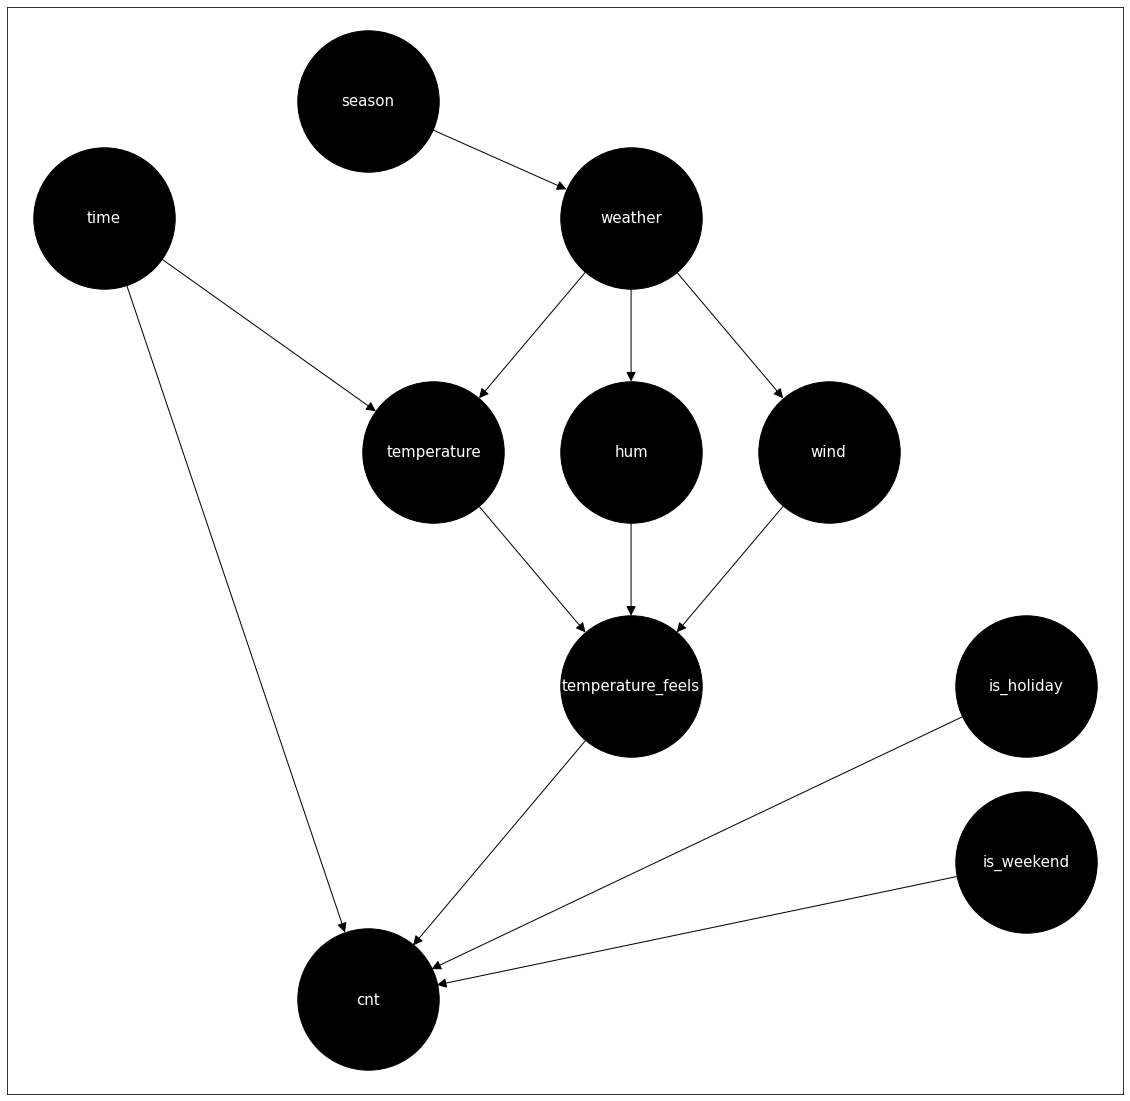
\includegraphics[width=0.6\textwidth]{network.png}
  \caption{The Network structure}
  \label{fig:net}
  \end{wrapfloat}

\paragraph{Generation of CPDs}
Since it wouldn't have been feasible to manually define the CPD Tables for variables with large
domain, we developed a function devoted to generate the table of conditioned probabilities associated
to a specific variable, according to its dependencies, represented by its parents.

\section{Exact Inference}

The basic task for any probabilistic inference system is to compute the posterior
 probability distribution for a set of query variables, given some observed event. Therefore, 
 given a set of evidence variables E and a query variable X a typical query asks for the posterior probability distribution 
\begin{equation}
P(X| e) = \frac{P(X, e)}{P(e)} = \alpha P(X| e) 
\end{equation}
Unfortunately, inference is a very challenging task: for many probabilities of interest, 
answering to any of these queries exactly is a NP-hard problem. However, the Variable 
Elimination Algorithm allows a more efficient computation, basing on the simple idea of
 performing calculations once and saving results for later use. To exploit this 
 efficient strategy we use the \texttt{pgmpy} class \texttt{VariableElimination}
and we performed some queries on the corresponding object. For example, a query was 
about the number of bikes that would be rented if the season is winter, the temperature is low, 
it is windy and rainy. Therefore, the evidence $E$ is $E = \{temperature = [-1, 7.75], wind = yes, weather = rain, season = winter\}$.
In Table~\ref{tab:exact-inference} there are the results of this query.

\begin{table}
  \centering
  \begin{tabular}[]{l r}
    \hline
    \textbf{cnt} & \textbf{p(cnt $|$ E)}\\
    \hline
    [47, 473] & 0.2583 \\
    (473, 753] & 0.1790 \\
    (753, 992] & 0.1720 \\
    (992, 1256] & 0.0925 \\
    (1256, 1595] & 0.0866 \\
    (1595, 2066] & 0.0881 \\
    (2066, 2762] & 0.0629 \\
    (2762, 7860] & 0.0605 \\
    \hline
  \end{tabular}
  \caption{Result of exact inference query}
  \label{tab:exact-inference}
\end{table}


\section{Approximate Inference}
Given the intractability of exact inference in large and multiple connected networks,
it turns out essential to consider approximate methods. In this report we examined two Direct
Sampling methods: the Rejection Sampling and the Likelihood weighting algorithm. 
To implement approximate inference we used the \texttt{pgmpy} class \texttt{BayesianModelSampling}. 



\subsection{Rejection Sampling}
\label{sec:rs}
To compute the approximate probability $\widehat{P}(X| e)$ the Rejection Sampling technique
generate samples and reject those that are not consistent with the evidence \textit{e}.
After generating all the samples that match the evidence, the algorithm compute the
approximate probability $\widehat{P}(X| e)$ as the ratio between the number of times in which the X occurs
in the samples and the total number of samples:
\[
\widehat{P}(X| e)= \frac{N_{PS}(X, e)}{N_{PS}(e)} \approx \frac{P(X, e)}{P(e)} = P(X| e)
\]
If the probability of the evidence $P(e)$ is small, Rejection Sampling can be very expensive, because it generates a lot of samples and rejects most of them.

\subsection{Likelihood Weighting}
\label{sec:lw}
The Likelihood Weighting technique avoids the inefficiency of Rejection Sampling by generating 
only events that are consistent with the evidence \textit{e}.
Each event is weighted by the likelihood of the event according to the evidence:
an event in which the evidence appears unlikely is given less weight\footnote{Artificial Intelligence. A Modern Approach, by Stuart Russel and Peter
Norvig, 3rd Ed.}. Therefore, to compute $\widehat{P}(X| e)$, the algorithm sums the weights 
of samples in which X occurs and divides the result by the sum of all the weights.

\subsection{Comparing the different methods}
We generated several sets of samples of different dimension according to the two 
 strategies using the \texttt{pgmpy} 
methods \texttt{rejection\_sample} and \texttt{likelihood\_weighted\_sample}. Afterwards, 
we computed the approximate probabilities as reported in Sections~\ref{sec:rs} and~\ref{sec:lw}.\\

We consider two queries:
 \begin{itemize}
   \item Query 1: which is the probability that $time = evening$ if $cnt = 3$ and $
    temperature = 1$?
   \item Query 2: which is the probability that  $cnt = 3$ if $
   temperature = 1$?\\
 \end{itemize}
 In Figure~\ref{fig:prob} we report how the approximate probabilities change varying the size of the
  set of samples for the two queries using Exact and Approximate Inference.\\

\begin{figure}[h]
\centering
{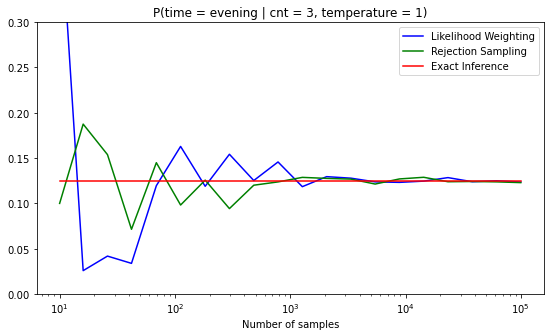
\includegraphics[width=.45\textwidth]{q1.png}} 
\quad{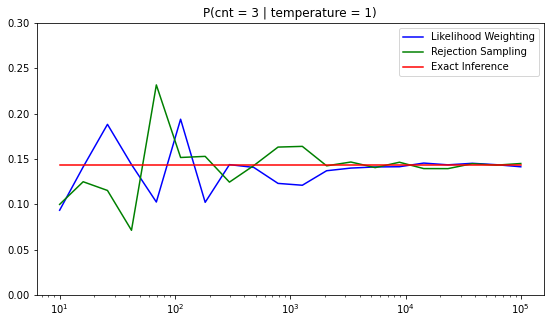
\includegraphics[width=.45\textwidth]{q2.png}} \\
\caption{Probabilities using exact and approximate inference}
\label{fig:prob}
\end{figure}

\section{Conclusions}
We can observe that increasing the number of samples the approximate probabilities
become closer and closer to the exact ones. In fact, as we can see in 
Figure~\ref{fig:error}, increasing the number of samples
the absolute and relative error become closer and closer to zero.

\begin{figure}[p]
  \centering
  {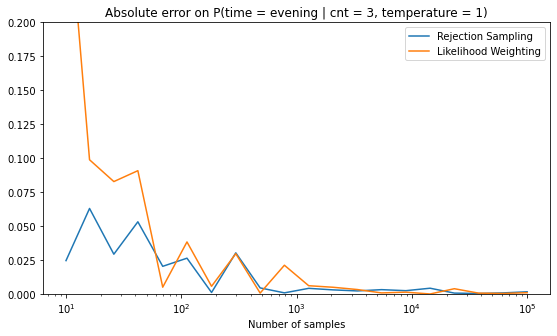
\includegraphics[width=.45\textwidth]{ab_err.png}} \quad
  {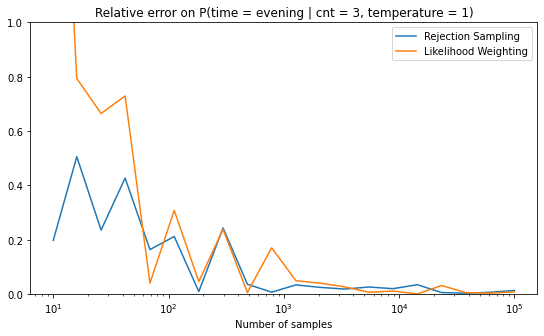
\includegraphics[width=.45\textwidth]{rel_err.png}} \\
  \caption{Absolute and Relative errors for the first query}
  \label{fig:error}
  \vspace{128in}
  \end{figure}


\end{document}